\chapter{Resultados da infraestrutura}
%Foi possível demonstrar uma aplicação que escala sob demanda
%Foi apresentada uma arquitetura que é possível de ser aplicada em produção

\section{Uso da infraestrutura}

A escolha da infraestrutura para a solução final foi o uso da
computação em nuvem (\autoref{infraestrutura-em-nuvem}), visto que, proporciona
escalabilidade que o problema exige - uma das principais vantagens da computação em nuvem.
Além é claro, do baixo custo inicial que a aplicação terá antes de começar a gerar qualquer
tipo de lucro.

Conforme discutido a respeito das topologias das plataformas em
nuvem (\autoref{tipologia-das-plataformas-em-nuvem}), para a solução final foi escolhido o
modelo IaaS (\autoref{iaas}) que fornece a opção de rodar programas como Docker e
Kubernetes, tornando a escolha do serviço de plataforma em nuvem independente da forma
com que o software roda. Ou seja, há um desacoplamento da infraestrutura com o software
(\autoref{ferramentas}).

\section{Análise de desempenho}

Foram feitos vários testes em cima do serviço de reserva de ingressos que foi implementado
(\autoref{implementacao-do-servico}) para saber quais eram seus limites.
É importante deixar claro que a análise ocorreu em um notebook pessoal com poder
de processamento limitado, conforme descrito no
\autoref{anexo-especificacao-de-hardware-do-servidor}.
Em um ambiente real (nuvem \autoref{infraestrutura-em-nuvem})
poderão existir diversas máquinas disponíveis para que sejam utilizadas
(escalabilidade horizontal \autoref{escalabilidade})
permitindo que o desempenho do sistema seja maior para atender muitas requisições.

\subsection{Gatling: ferramenta para geração da análise de desempenho}

Os testes de performance realizados em cima da aplicação de reserva de ingressos foram
feitos com a ferramenta Gatling na versão 2.3.
Com a ferramenta é possível testar alta performance de aplicações web
\cite{gatling-docs} que seguem o protocolo HTTP.

\subsection{Gráficos da análises de desempenhos}

O teste de performance de requisições foi feito usando a
estratégia do método heavisideUsers \cite{gatling-simulation-setup}
que o Gatling possui, simulando assim a utilização simultânea do sistema por
grande quantidade de usuários.
As requisições da análise da
\autoref{03000-requests-config-10s-duration-10},
\autoref{05000-requests-config-10s-duration-10}
e \autoref{10000-requests-config-10s-duration-13}
foram configuradas para serem executadas no período de 10 segundos.
Os testes foram feitos para medir a degradação do sistema em relação ao aumento do
número de requisições simulando um ambiente onde haveriam muitas requisições para
reserva de ingressos.
Com a degradação do sistema as respostas começam a demorar mais, ou seja,
o teste demora mais para ser finalizado conforme o aumento do número de requisições.
Com isso, o único parâmetro que muda de um teste para o outro
é o número de requisições realizadas.

Na requisição é possível informar a quantidade de ingressos.
Nos testes realizados todas as requisições fazem a solicitação da reserva de
2 ingressos e o evento está configurado para 100.005 ingressos disponíveis.

Na \autoref{03000-requests-config-10s-duration-10} são feitas 3.000 requisições apenas.
O sistema responde todas elas com sucesso e um desvio padrão de 241 milissegundos
para o tempo de resposta das requisições.
97\% das requisições respondem em menos de 800 milissegundos e apenas 3\% das requisições
respondem em até 1.200 milissegundos.

\begin{figure}[h]
  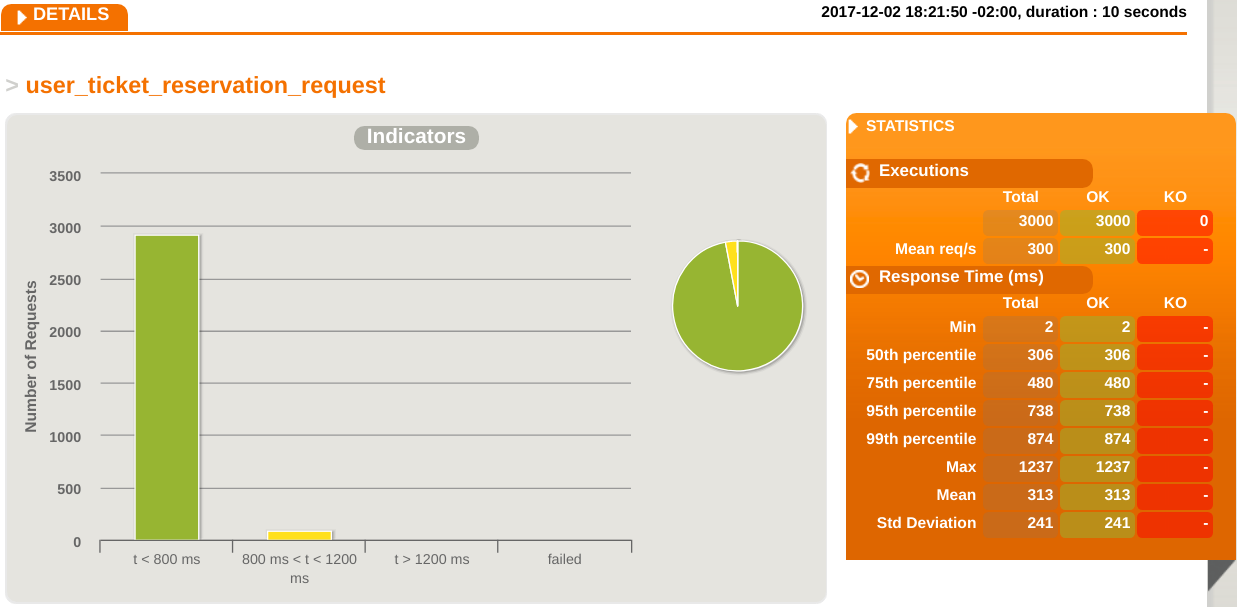
\includegraphics[width=\textwidth]{03000-requests-config-10s-duration-10}
  \caption{Dados do Gatling com 3.000 requisições executados em 10 segundos}
  \label{03000-requests-config-10s-duration-10}
\end{figure}

Na \autoref{05000-requests-config-10s-duration-10} são feitas 5.000 requisições.
O sistema responde todas elas com sucesso e um desvio padrão aumenta para 569 milissegundos
para o tempo de resposta das requisições.
78\% das requisições respondem em menos de 800 milissegundos, 18\% das requisições
respondem em até 1.200 milissegundos e apenas 4\% das requisições
respondem com tempo maior que 1.200 milissegundos.

\begin{figure}[h]
  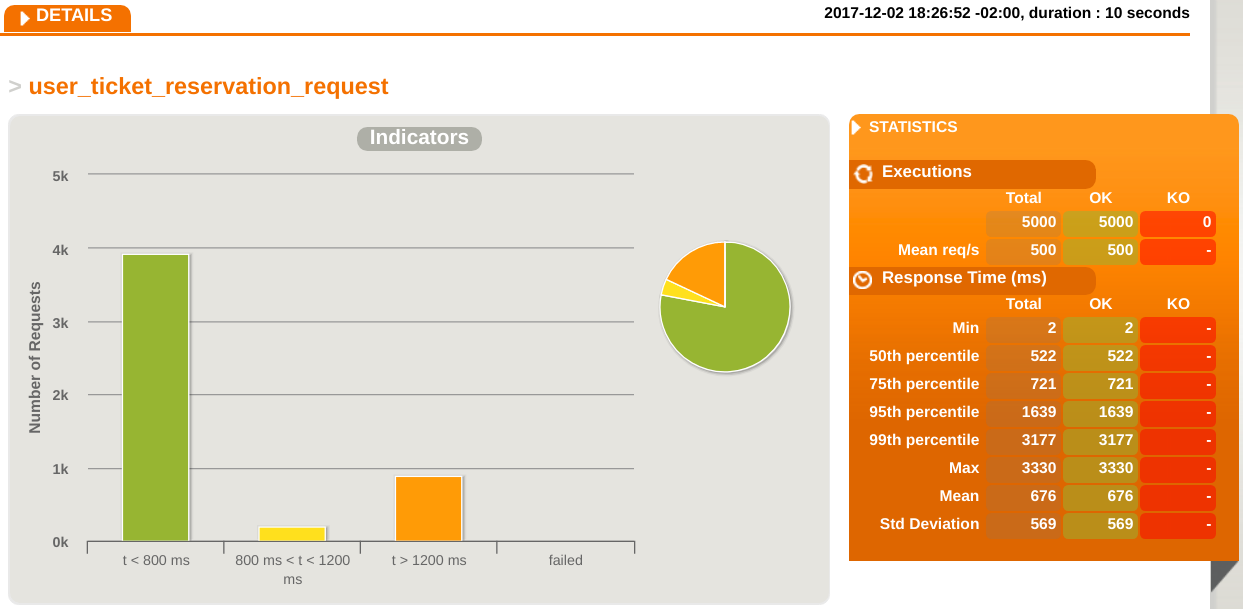
\includegraphics[width=\textwidth]{05000-requests-config-10s-duration-10}
  \caption{Dados do Gatling com 5.000 requisições executados em 10 segundos}
  \label{05000-requests-config-10s-duration-10}
\end{figure}

Na \autoref{10000-requests-config-10s-duration-13} são feitas 10.000 requisições.
O sistema responde todas elas com sucesso e um desvio padrão aumenta para 1.117 milissegundos
para o tempo de resposta das requisições.
5\% das requisições respondem em menos de 800 milissegundos, 3\% das requisições
respondem em até 1.200 milissegundos e 93\% das requisições
respondem com tempo maior que 1.200 milissegundos. Aqui fica claro que há grande
degradação do sistema quanto ao tempo de resposta. Porém,
todas as requisições foram atendidas.

\begin{figure}[h]
  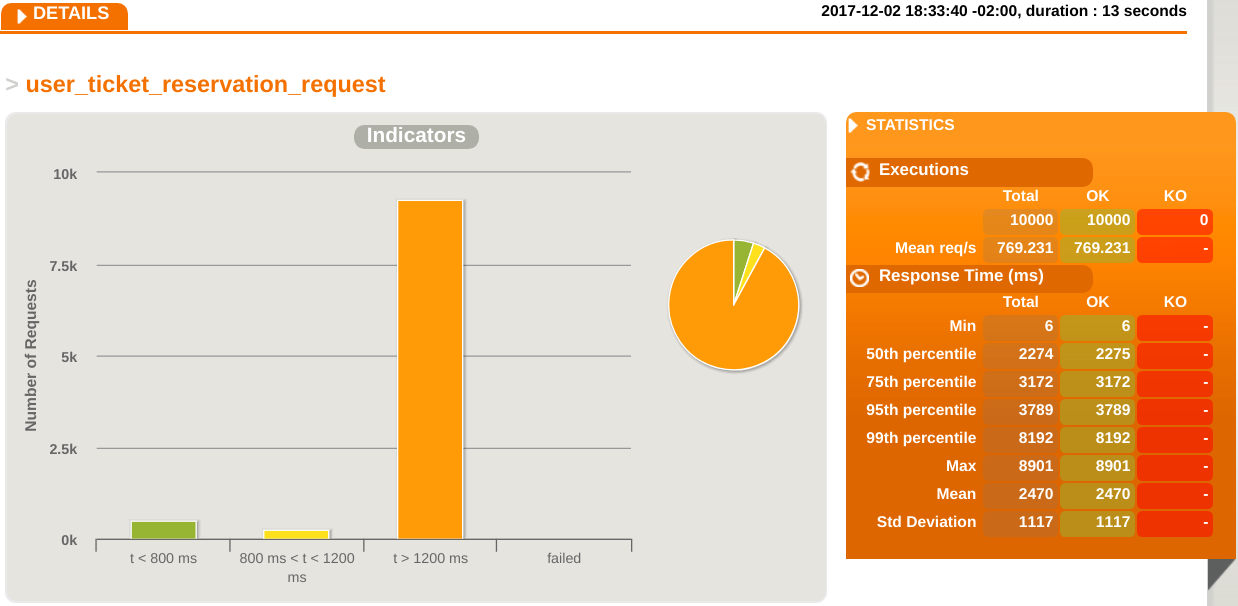
\includegraphics[width=\textwidth]{10000-requests-config-10s-duration-13}
  \caption{Dados do Gatling com 10.000 requisições executados em 13 segundos}
  \label{10000-requests-config-10s-duration-13}
\end{figure}

A \autoref{28000-requests-config-30s-duration-34} possui o tempo de teste configurado
com 30 segundos de execução.
O que se pode concluir com os dados analisados é que a aplicação consegue atender
em torno de 28.000 requests com sucesso em 34 segundos com desvio padrão de
4.111 milissegundos.
O tempo de respostas é considerado alto - imaginando um usuário aguardando em
torno de 5 segundos para saber se sua reserva foi realizada.
Porém, a solicitação da reserva é atendida.

\begin{figure}[h]
  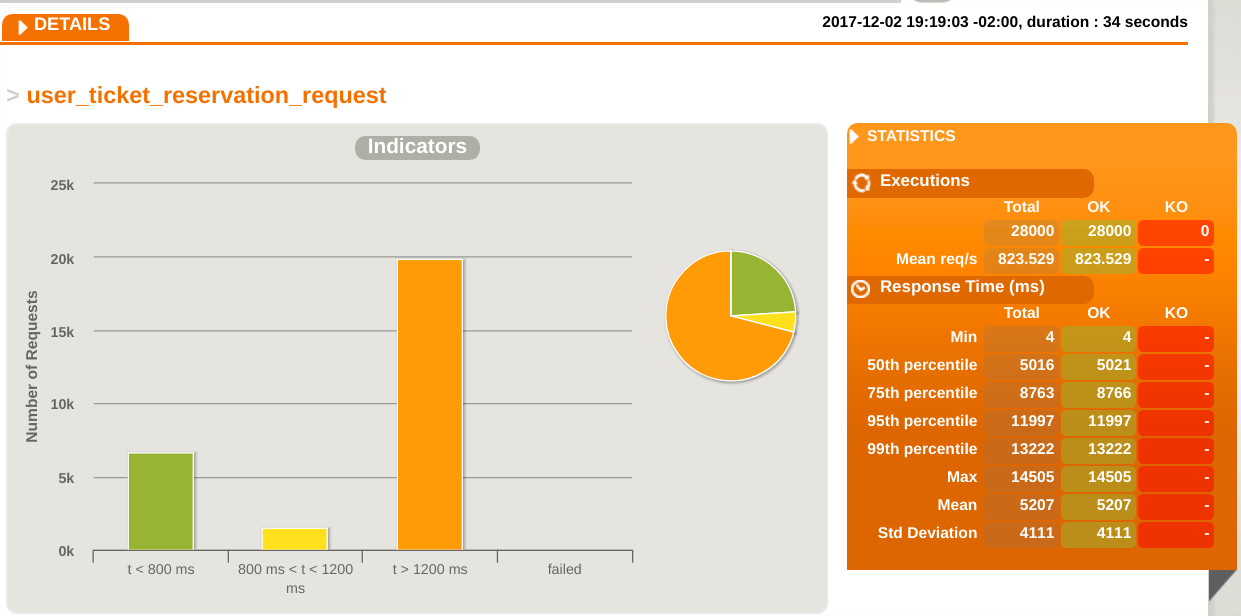
\includegraphics[width=\textwidth]{28000-requests-config-30s-duration-34}
  \caption{Dados do Gatling com 28.000 requisições executados em 34 segundos}
  \label{28000-requests-config-30s-duration-34}
\end{figure}

A \autoref{30000-requests-config-10s-duration-33} possui o tempo de teste configurado
com 10 segundos de execução.
O que se pode concluir com os dados analisados é que a aplicação consegue atender
em torno de 28.000 requests com sucesso em 33 segundos com desvio padrão de
5.766 milissegundos.
O tempo de resposta aumenta mais ainda.
Comparando com a \autoref{28000-requests-config-30s-duration-34}, é possível ver
que a quantidade de respostas sem erros no servidor chega ao seu limite.
A partir das 28.000 requests o servidor começa a ter problemas de conexão.

\begin{figure}[h]
  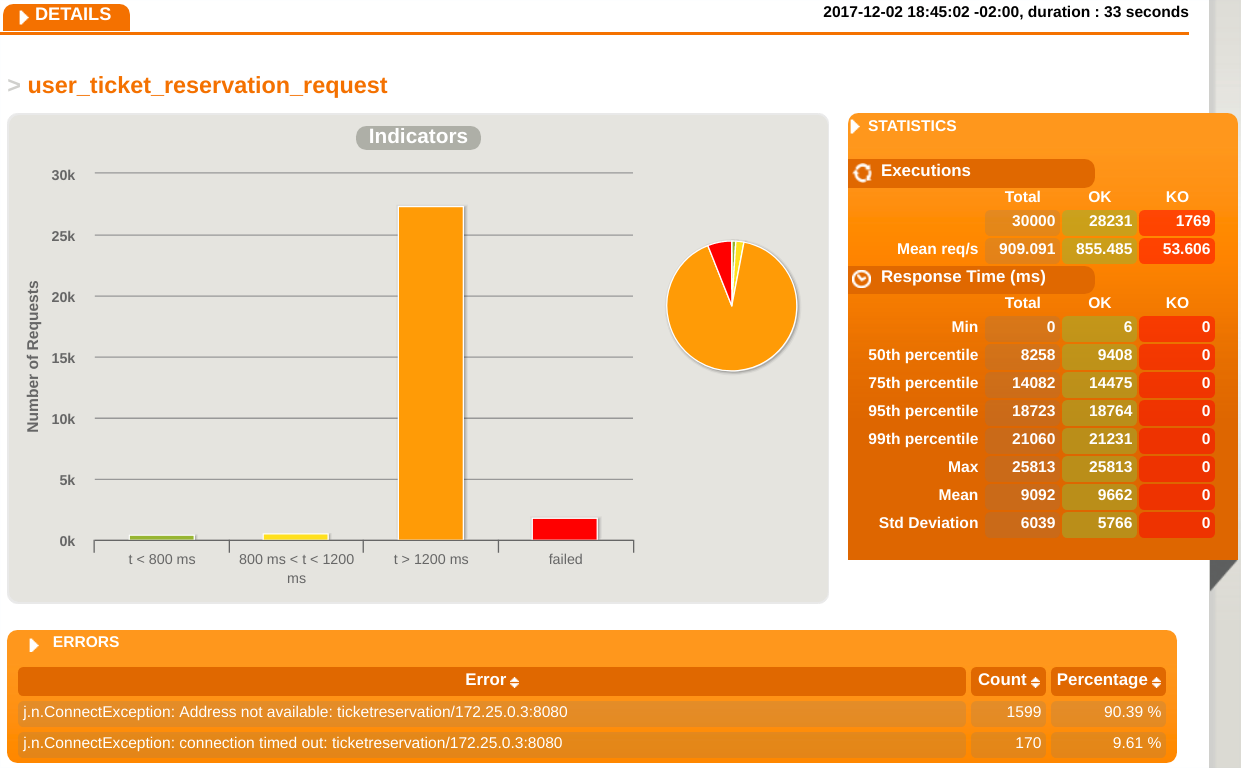
\includegraphics[width=\textwidth]{30000-requests-config-10s-duration-33}
  \caption{Dados do Gatling com 30.000 requisições executados em 33 segundos}
  \label{30000-requests-config-10s-duration-33}
\end{figure}

Com a escalabilidade horizontal é possível começar a expandir esse poder de processamento.

Todos os resultados com todos os testes realizados podem ser consultados de maneira
iterativa através do link \url{https://andreformento.github.io/term-paper/index.html}.
